%!TEX root = P231_notes.tex

\section{Green's functions in diverse dimensions}
% \lecdate{lec~12}
% 2018 Lec 27

For most graduate courses, we we examine simple examples where we can focus on understanding the physics. We then leave it to you to generalize to the horrible real-world scenarios that you'll encounter in your other graduate courses and research. There's one generalization that we should take time to do properly together: the shift from one dimension to multiple dimensions. This is the shift from working with functions of time to functions \emph{spacetime}. Equivalently, the harmonic oscillator converts into a wave.
%
Keep in mind that we're not doing any special relativity, even though we'll borrow notation from special relativity\footnote{There was once a professor teaching electrodynamics who used notation informed by relativity. Some of the condensed matter students complained the class is about electricity and magnetism, not relativity. The professor replied: just where do you think magnetism comes from?}. 

\subsection{The `harmonic oscillator' in spacetime}
The second derivative in higher-dimensional Euclidean space is the Laplacian, $\nabla^2= \partial_x^2 + \partial_y^2 +\cdots$. But when you combine space and time (Minkowski space), there's the famous relative minus sign\footnote{At this level the minus sign is a convenient convention, but we know that the second derivative should really be relativistically invariant: $\partial^2 = \partial_\mu \partial^\mu$.}:
\begin{align}
	\frac{d^2}{dt^2}
	\to 
	\frac{1}{c^2}
	\frac{\partial}{\partial t}^2
	-
	\frac{\partial^2}
	{\partial \vec x^2} \ ,
\end{align}
where $\partial/\partial\vec x = \nabla$ is the gradient. The overall sign is a convention. Against all of my hard-developed instincts for natural units, I have replaced the explicit value of $c$ so that the operator makes sense dimensionally: each term has powers of inverse length squared. In what follows I'm likely to make mistakes\footnote{My adviser used to say: if you think there may be a sign error or a factor of two error, then your homework is to fix those errors. In this case, if you think there's a missing factor of $c=1$, I'm not even sure if I'd even acknowledge that it's actually an error.} with the factors of $c$. 


In (1+1)-dimensions of spacetime\footnote{The (1+1) notation means one dimension of space, one dimension of time.} this is $\partial^2 = c^{-2} \partial_t^2 - \partial_x^2$. That looks familiar, doesn't it? The minus sign tells us that if we move forward in time a little bit, but look `backward' in space, then the function doesn't change. The description of the state at time $t-\delta t$ and position $x-\delta x$, subject to $\delta x = c\delta t$, is the same as the state at time $t$ and position $x$. 
%
This, in turn, means that the information was propagated \emph{forward} in space as time also moves forward. This is exactly what we expect from a wave. We recall that the solution to second derivative differential equations are usually trigonometric functions or their exponential counterparts. We further recall that `plane waves' are described with the same funny minus sign:
\begin{align}
	f(t) \sim \sin (\omega t - kx) \ .
	\label{eq:plane:wave}
\end{align}
From this you can read off that the plane wave velocity is $\omega/k$. Of course, you already knew that from dimensional analysis. 

\begin{exercise}
This is a great place to reflect on phase versus group velocity. I should probably write such a discussion into a future version of this notes. \flip{To do.} In the meanwhile, one of my favorite puzzles is the following (perhaps apocryphal) story.\footnote{I think I first heard this story from Tony Zee's lectures at the African School for Theoretical Physics in 2004. He posed this as an obvious problem in dimensional analysis. I don't think I properly appreciated the `obvious' aspect until about 15 years later while preparing this course. It wasn't completely obvious to me at all.} During the second world war, an admiral wanted to be able to use reconnaissance photographs of ships to determine their velocities. The admiral knew that given data about the ships' positions and velocities, one could extrapolate where those ships are going and when they will arrive. Because ships leave a wake behind them, the admiral figured that a clever physicist should be able to determine a ship's velocity based on the angle of the wake behind the boat.

In deep water, this is called a Kelvin wake. You also see this when watching ducks on the river.\footnote{Not everyone has a chance to watch battleships from a spy plane, but it turns out plenty of universities are situated near rivers where generations of the mathematically inclined could reflect on physical phenomena. I suspect this is the reason why Cambridge has such a historically strong fluid dynamics department. Anyway, I used to watch the ducks swimming in the stream near my old Ph.D institution. There were also geese around. I wouldn't watch the geese. I suspect they also leave a Kelvin wake, but I am quite sure that geese leave behind gigantic goose shits that make it unpleasant to sit by the water.} The key `aha' moment for understanding the Kelvin wake is that the relevant model is one where the key restoring force comes from gravity---these wakes are formed by \emph{gravity} waves. Do not confuse this with \emph{gravitational waves}, which are quite different. By neglecting surface tension, we find that the phase velocity is $\sqrt{g/k}$, where $k$ is the wave number ($e^{ikx}$). The group velocity (that carries energy) is $d\omega/dk$, where $\omega=\sqrt{gk}$ is the angular frequency. Thus the group velocity is half the phase velocity. 

Using a geometric argument, show that the angle of the Kelvin wake is $\sin^{-1}(1/3)$. The book by Stone \& Goldbart has a nice discussion.\footnote{See also \url{www.itp.uni-hannover.de/fileadmin/itp/emeritus/zawischa/static_html/KWake.html}} Even before jumping into the construction, you should wonder where the ratio 1:3 shows up in the problem. 
\end{exercise}
% A good exercise: phase and group velocity; see appell or cahill

\subsection{Green's functions for multidimensional spaces}
Our `harmonic oscillator' equation becomes:
\begin{align}
	\left[\frac{1}{c^2}
			\frac{\partial}{\partial t}^2
			-
			\frac{\partial^2}
			{\partial x^2}
			-
			\frac{\partial^2}
			{\partial y^2}
			-
			\frac{\partial^2}
			{\partial z^2}
		\right]
		\varphi(\vec{x},t) = \rho(\vec{x},t) \ .
		\label{eq:phi:wave:eq}
\end{align}
Huh, that looks familiar, doesn't it? We've chosen variables so that this looks just like the wave equation for the scalar potential $\varphi$ subject to a charged source $\rho$ in electrodynamics! In fact, you know how this works. There are three more equations that correspond to the vector potential:
\begin{align}
	\left[\frac{1}{c^2}
			\frac{\partial}{\partial t}^2
			-
			\frac{\partial^2}
			{\partial x^2}
			-
			\frac{\partial^2}
			{\partial y^2}
			-
			\frac{\partial^2}
			{\partial z^2}
		\right]
		\vec A(\vec{x},t) = \vec j(\vec{x},t) \ .
		\label{eq:A:wave:eq}
\end{align}
Now let's go through a series of questions about \eqref{eq:phi:wave:eq} and \eqref{eq:A:wave:eq} to make sure we're on the same page. 
\begin{enumerate}
\item \textbf{Are these differential equations still linear?} Yes. Remember what it means to be linear! $\mathcal O(f+g) = \mathcal Of +\mathcal Og$, for example.
\item \textbf{Are we worried that there are multiple arguments?} Not really. The functions now depend on $t$ and $\vec{x}=(x,y,z)$. You went from an infinite dimensional `vector space' to a still-infinite dimensional vector space\footnote{You can pontificate about whether this infinity is `bigger.' It doesn't really make a difference.}. You can also mumble reassuring words to yourself, perhaps recalling how in prior encounters with the wave equation you've perhaps separated your functions into single-argument factors, $\Psi(t,x) = T(t)X(x)$, or something like that.
\item \textbf{How many equations are there?} There are \emph{four}\footnote{Obligatory TNG reference: \url{https://www.youtube.com/watch?v=wjKQQpPVifY}} equations. There is an equation for $\phi$ and one equation for each component of $\vec A$. In fact, we typically bundle this all up into a four-vector $A_\mu=(\varphi, \vec A)$.\footnote{For now this is just a bundling, so you may argue that it's not obviously a \emph{vector}. The fact that $\varphi$ and $\vec{A}$ transform into each other upon performing a boost is something we learn from physical observations. Alternatively, the identity of $A_\mu$ as a vector (technically, a one-form) is imposed by the mathematical structure---but that mathematical structure was adopted after the empirical progress in the 1800s.}
\item \textbf{How many differential operators are there?} Just one. There is only \emph{one} differential operator, $\partial^2$. It acts on different components of $A_\mu$, but it's the same wave operator acting on each component. 
\item \textbf{... so how many equations are there, really?} All four equations are essentially the same equation with different state functions and different sources. So it's really just one class of differential equation.
\end{enumerate}
Okay, here's the really important one. I'm going to put it in a box to make sure you pay really close attention. Please answer the following question before reading on:
\begin{framed}
\centering
How many Green's functions are there?
\end{framed}
Do we need a Green's function for each component of $A_\mu$? Do we need a Green's function for each dependent variable, $x^\mu = (ct,x,y,z)$? \emph{No}! There is only \emph{one} differential equation, and thus there is only \emph{one} Green's function. 

Let's see how this works. Suppose you have a differential equation in multiple variables,
\begin{align}
	\mathcal O_\vec{x} f(\vec{x}) = s(\vec{x}) \ .
\end{align}
Let's say that $\vec{x}=(x_1, \cdots, x_N)$, so that we're working in $N$-dimensional space. Suppose you are given the Green's function $G(\vec{x},\vec{x}')$ for $\mathcal O_\vec{x}$. This means that $G$ satisfies the Green's function equation
\begin{align}
	\mathcal O_\vec{x} G(\vec{x},\vec{x}') = \delta^{(N)}(\vec{x}-\vec{x}') \ ,
\end{align}
where the $N$-dimensional $\delta$-function is simply the product of one-dimensional $\delta$-functions in the expected way:
\begin{align}
	\delta^{(N)}(\vec{x}-\vec{x}') 
	&=
	\delta(x_1-x_1')\delta(x_2-x_2')\cdots\delta(x_N-x_N') \ .
\end{align}
The solution to the above differential equation is
\begin{align}
	f(\vec{x}) &= \int d^N\vec{x}'\,  G(\vec{x},\vec{x}') s(\vec{x}') \ ,
\end{align}
which you can check by acting on both sides with $\mathcal O_\vec{x}$.

\subsection{Relativistic Notation}

Let's borrow some four-vector notation from special relativity. Nothing that we're doing is based on special relativity, but the fact that it pops out for free is telling. Our indices $\mu$ run over four values which we take to be $\mu = 0,1,2,3$ corresponding to timelike (0) and spacelike (1,2,3) directions. Some objects are naturally defined with an upper index, like $x^\mu = (ct,x,y,z)$. You can lower these indices using the metric, $\eta_{\mu\nu}=\text{diag}(1,-1,-1,-1)$. This means that for some vector $v^\mu$,
\begin{align}
 	v^2 \equiv v^\mu v_\mu 
 	= c^2(v^0)^2 - (v^1)^2 - (v^2)^2 - (v^3)^2 \ .
 \end{align}
 More importantly, this means that the four-vector of partial derivatives, which is naturally a lower-index object, squares to:
 \begin{align}
	 \partial^2\equiv
 	\partial_\mu \partial^\mu 
 	&= 
 	\frac{1}{c^2}
			\frac{\partial}{\partial t}^2
			-
			\frac{\partial^2}
			{\partial x^2}
			-
			\frac{\partial^2}
			{\partial y^2}
			-
			\frac{\partial^2}
			{\partial z^2} \ .
 \end{align}
The placement of the $c^2$ factors should be clear from dimensional analysis. We see that indeed the wave operator is the natural generalization of the harmonic oscillator in spacetime. We won't actually be raising and lowering indices, but we want to be clear that there's a natural `dot product' that includes the relative minus sign between spatial and temporal components.

The states and sources in our system are the (four-)vector potential $A_\mu$ and the current $j_\mu$: 
\begin{align}
	A_\mu &= (\varphi, \vec{A})
	&
	j_\mu &= (\rho, \vec{j}) \ .
\end{align}
The four equations for the vector potential are
\begin{align}
	\partial^2 A_\mu = j_\mu \ .
\end{align}
That's one equation for each value of $\mu$, but each equation has the \emph{same} differential operator $\partial^2$. Our task is to find the Green's function for this operator in spacetime. The Green's function equation is
\begin{align}
	\partial^2 G(x,x') &= \delta^{(4)}(x-x') \ ,
	\label{eq:wave:eq:Greens:eq}
\end{align}
where we write $x$ and $x'$ to mean \emph{four}-vectors with \emph{components} $x^\mu$ and $(x')^\mu$. Given a current $j_\mu(x)$, the vector potential is the solution to the wave equation which integrates over all of the current (source) positions:
\begin{align}
	A_\mu(x) &= \int d^4x' \, G(x,x') j_\mu(x) \ .
\end{align}
Observe that $G$ has two arguments, $x$ and $x'$, but no indices. The two arguments correspond to the observation point $x$ and the source point $x'$. The integral over $d^4x'$ means we're accounting for sources from all positions and all times\footnote{This should remind you of starlight that is emitted a long time ago ($t'$) in a galaxy far, far away ($\vec{x}'$ that we we observe today $(t,x)$.}. We haven't specified our choice of coordinates. For now you can assume that we are using Cartesian coordinates, but you may recall that the Green's function for the Poisson equation\footnote{Which we can now call the `harmonic oscillator' in (3+0)-dimensional spacetime.} is most cleanly expressed in spherical coordinates, $G(r)\sim (4\pi r)^{-1}$. You should expect that the natural way to write $G(x,x')$ in (3+1)-dimensional spacetime is some hybrid of spherical and Cartesian coordinates.

\begin{exercise}\label{ex:guess:Greens}
At this point you may want to start going over Homework \#4 where \emph{you} solve the (3+1)- and (2+1)-dimensional Green's functions in detail. I'm quite proud of that homework assignment, there's a lot of neat observations. One observation is that with some physical insight, you could take the Poisson equation's Green function and \emph{guess} the Green's function for the wave equation simply by using the finite speed of light. This is discussed nicely in Tony Zee's latest textbook, \emph{Fly By Night Physics}. 
\end{exercise}


We solve \eqref{eq:wave:eq:Greens:eq} in what is now the `usual' way. We Fourier decompose both sides. Making deliberate choices for our Fourier transform conventions, let us write
\begin{align}
	f(t,\vec{x}) &= \int \dbar^4k \, e^{-ik\cdot x} \tilde f(\omega, \vec{k})
	&
	\dbar^4k &= \frac{dE\, d^3\vec{k}}{(2\pi)^4}
	 \ .
\end{align}
\begin{exercise}
Please confirm that with our metric convention, this choice of (3+1)-dimensional Fourier conventions matches the (0+1)-dimensional Fourier conventions we used for the harmonic oscillator.
\end{exercise}
For simplicity we'll just write $f(x)$ and $\tilde f(k)$ to refer to the four-component arguments\footnote{Later on we'll use $k=|\vec{k}|$ to mean the spatial length of the 3-momentum; there should be no ambiguity because the context should be clear. This is an example of `read what I mean, not what I [literally] write.' This is a common `chalkboard physics' peccadillo; usually it's a pain to write \emph{literally} what you mean. Sometimes it's better to write the `easy to interpret' equation, then tell people to interpret it slightly differently. Mathematicians should be incensed. That's okay. This is mathematics for physicists, not physics for mathematicians. The latter course is also quite interesting and theorists should take it if it's ever offered from John Baez.}. 
We have used the Minkowski spacetime inner product,
\begin{align}
	k_\mu x^\mu \equiv k\cdot x = Et - \vec{k}\cdot\vec{x} \ .
\end{align}
From the perspective of the Fourier transform, this is just a sign convention for each Cartesian direction that we are free to make. From the perspective of physics, we know that it is convenient to pick a notation that is manifestly Lorentz invariant\footnote{If we had chosen a different notation, the theory would still be Lorentz invariant---its built into the operator---but it would not be \emph{obviously} Lorentz invariant. This would be like using cylindrical coordinates and losing track about whether or not space is rotationally symmetric.} and automatically looks like a traveling wave. By the way, if you're keeping track of factors of $c$:
\begin{align}
	x^\mu &= (ct,\vec{x})
	&
	k^\mu &= (E/c,\vec{p})
	&
	k_\mu &= (E/c, -\vec{p})
	&
	x\cdot k  &= Et - \vec{p}\cdot\vec{x} \ .
\end{align}
I hate keeping track of factors of $c$. 


Here's what the Fourier transform of the spacetime $\delta$-function looks like:
\begin{align}
	\delta^{(4)}(x-x') &=
	\int \dbar E e^{-iE(t-t')}
	% \times
	\int \dbar k_x e^{+ik_x(x-x')}\
	% \times
	\int \dbar k_y e^{+ik_y(y-y')}\
	% \times
	\int \dbar k_z e^{+ik_z(z-z')} \ .
\end{align}
Again, we have \emph{chosen} the sign of the Fourier transform so that the time-like component has a minus sign, $e^{-iE(t-t')}$, while the space-like component has a plus sign, $e^{+ik_x(x-x')}$. This is convenient since we could package all of these exponential together with respect to $k_\mu = (E, -k_x, -k_y, -k_z)$,
\begin{align}
	\delta^{(4)}(x-x') &=
	\int \dbar^4k e^{-ik\cdot (x-x')} \ .
	\label{eq:4D:delta:Fourier}
\end{align}
Conveniently, this looks just like a---\emph{wait for it}---plane wave:
\begin{align}
	e^{-ik\cdot x} = e^{-i\left(Et - \vec{k}\cdot\vec{x}\right)} \ .
\end{align}
Compare this to \eqref{eq:plane:wave}. By the way, if you're really picky you can bring up factors of $c$ again because you argue that $\delta(t-t')$ should really be $\delta(ct-ct')$. This is worth checking, but I'd rather relegate it to yet another parenthetical footnote\footnote{
	If we keep factors of $c$ explicit, then we recall that $t\to ct$ and $E\to E/c$. The expression $\delta(t-t')$ is replaced by $\delta(ct-ct') = \delta(t-t')/c$. The factor of $1/c$ shows up in the corresponding replacement $dE \to dE/c$. To solve for the Fourier transform $\tilde G$, we compare Fourier coefficients of the $\delta$ function with the Fourier coefficients of the Green's function. In that comparison, these factors of $c$ cancel out. Thus we are free to simply write $\delta(t-t')$ as long as our integration measure is $dE$ and not $dE/c$. If you're ever lost, you should just set $c=1$ and then replace factors of $c$ at the end to make sure the dimensions of $G$ work out.
}.

The left-hand side of the Green's function equation \eqref{eq:wave:eq:Greens:eq} is 
\begin{align}
	\partial^2 \int \dbar^4k \, e^{-ik\cdot x} \tilde G(k,x')
	&=
	\int \dbar^4k \, \left(-\bar{E}^2+\vec{k}^2\right) e^{-ik\cdot x} \tilde G(k,x')
	&
	\bar{E}\equiv E/c
	 \ .
	\label{eq:4D:Greens:wave:LHS:Fourier}
\end{align}
We have introduced the $\bar E$ notation to keep track of the factors of $c$ coming from $\partial^2 \sim c^{-2}\partial_t^2 -\cdots$. If you'd had set $c=1$, you could have guessed this because you want to make sure that both terms in the denominator have the same dimensions.
Equating the Fourier coefficients of \eqref{eq:4D:delta:Fourier} with \eqref{eq:4D:Greens:wave:LHS:Fourier} gives us the Fourier modes:
\begin{align}
	\tilde G(k,x') &= \frac{-e^{ikx'}}{\bar{E}^2 - \vec{k}^2} \ .
\end{align}
Thus the wave equation Green's function in (3+1)-dimensions is:
\begin{align}
	G(x,x') &= \int \dbar^4k \, \frac{-e^{ik\cdot (x-x')}}{\bar{E}^2 - \vec{k}^2} \ .
	\label{eq:Greens:function:For:4D:int}
\end{align}
This looks almost trivial---you've integrated something with this \emph{exact} integrand before when we did the harmonic oscillator. The only issue is that now the $\dbar\omega$ has been replaced with a much more\footnote{\emph{The more integrals we come across, the more problems we see}, with apologies to the Notorious \acro{BIG}.} ominous $\dbar^4k$. 

\subsection{Sketch of the Fourier integral in (3+1)-dimensions}

Rather than solve this in gory detail, we'll just provide the framework and then we'll it to you to dot all the $i$s and cross all the $t$s.  It'll be a little tedious the first time you do do this integral, but don't worry. If you drink alcohol, I recommend a glass of wine\footnote{Or the appropriate substance relevant for you personally.} before starting.

The solution is most clear if we use \textbf{hypercylindrical} coordinates that correspond to spherical coordinates over the spatial directions and a Cartesian coordinate in the time direction. The integration measure is
\begin{align}
	\dbar^4k &= \frac{1}{(2\pi)^4} dE \, |\vec{k}|^2 d|\vec{k}|\, d\cos\theta \, d\varphi \ .
	\label{eq:4D:momentum:measure}
\end{align}
The polar angle $\theta$ is defined by 
\begin{align}
	(\vec{x}-\vec{x}')\cdot \vec{k} = |\vec{x}-\vec{x}'||\vec {k}| \cos\theta \ .
\end{align}

\paragraph{The azimuthal integral.}
The azimuthal angle $\varphi$ is defined with respect to the azimuthal direction set by $\vec{x}-\vec{x}'$. Observe that the integrand of the Fourier integral \eqref{eq:Greens:function:For:4D:int} is completely independent of $\varphi$ so we might as well do the $d\varphi$ integral first:
\begin{align}
	\int_0^{2\pi} \dbar \varphi &= 2\pi \ .
\end{align}
This conveniently cancels a factor of $(2\pi)$ in the denominator of \eqref{eq:4D:momentum:measure}.

\paragraph{The polar integral.}
We can tidy up our remaining expressions by defining $c=\cos\theta$ and $k = |\vec{k}| = \sqrt{k_x^2 + k_y^2+k_z^2}$ for the radial direction in momentum space; hopefully this doesn't cause any ambiguity with $k = (E/c,k_x,k_y,k_z)$ the four-vector\footnote{It will not cause any ambiguity because you'll notice that all of the factors of $c$ have been removed in the Fourier integrand \eqref{eq:Greens:function:For:4D:int}.}. Similarly, let's write $r$ to be the separation distance between the observer and the source, $r=|\vec{x}-\vec{x}'|$. Thus we have
\begin{align}
	\int_{-1}^1 d\cos\theta \, e^{i\vec{k}\cdot(\vec{x}-\vec{x'})}
	&=
	\int_{-1}^1 dc\, e^{ikrc}
	= 
	\frac{1}{ikr}\left(e^{ikr} - e^{-ikr}\right) \ .
\end{align}
Plugging this into \eqref{eq:Greens:function:For:4D:int} gives
\begin{align}
	G(x,x') &=
	\frac{1}{(2\pi)^3}
	\int dk \, dE \, k^2
	\, 
	\frac{1}{ikr}\left(e^{ikr} - e^{-ikr}\right)
	\frac{- e^{-iE (t-t')}}{\bar{E}^2-k^2}
	\\
	&=
	\frac{1}{8\pi^3 ir}
	\int_0^\infty dk\, 
	k \left(e^{ikr} - e^{-ikr}\right)
	\int_{-\infty}^\infty dE \, 
	\frac{-e^{-iE (t-t')}}{\bar{E}^2-k^2}
	\ .
\end{align}
For simplicity we have renamed $|\vec k| \to k$. Note the limits of the integrals. Because $k$ is a radial variable, it only takes non-negative values. The energy integral, on the other hand, is an honest Fourier transform over all real values.

\paragraph{The energy integral.} Ah! The $dE$ integral is an old friend: you remember it when it used to go by the name $d\omega$ for the harmonic oscillator. You know how to do this one: just follow what we did to derive the retarded Green's function for the harmonic oscillator. Nudge the poles infinitesimally into the lower-half plane\footnote{This is as good a time as any to point out that the rule of nudging the poles into the \emph{lower} half plane for the causal propagator is directly related to our Fourier integral convention. Some references use the opposite convention and thus nudge the poles into the upper half plane.}. The solution is
\begin{align}
	 \frac{1}{2\pi}\int_{-\infty}^\infty dE \, 
	\frac{-e^{-iE \Delta t}}{\bar{E}^2-k^2}
	&= \frac{-i}{2k}\left(e^{ikc\Delta t} - e^{-ikc\Delta t}\right)\Theta(\Delta t) \ .
\end{align}
Note that we have been careful to replace the factors of the speed $c$ when integrating since we remember $\bar E \equiv E/c$. This is straightforward from writing $E = c\bar E$ and then changing integration variables $dE = cd\bar{E}$. You could have also guessed this because you know the right-hand side will have exponentials with arguments that go like $k$ and $\Delta t$. In order for these to make sense dimensionally, there must be a factor of $c$ in there\footnote{If you're being strict about units, recall that the `energies' are really frequencies and the `three-momenta' are really wave numbers. Those who like to think in natural units will be confused why this footnote is necessary.}.

Compare this to \eqref{eq:HO:Gret:sin:theta}. We have chosen not to write the difference of exponentials into sines; we will see why shortly. Otherwise, the three-momentum magnitude $k$ plays the role of the frequency $\omega_0$. We went ahead and wrote $\Delta t \equiv t-t'$; in the harmonic oscillator we equivalently said\footnote{Technically we said $t_0=0$ because that subscript made sense for an `initial time,' but now we use a more standard Green's function convention that $x'$ is the spacetime position of the source.} ``set $t'=0$''. 

\paragraph{The [magnitude of the] three-momentum integral.} The remaining integral over $k=|\vec k|$ is
\begin{align}
	G(x,x')&= -
	\frac{\Theta(\Delta t)}{8\pi^2 r} 
	\int^\infty_0
	dk\, 
	\left[
 		e^{ik(r+c\Delta t)}
 		- e^{ik(r-c\Delta t)}
 		- e^{ik(-r+c\Delta t)}
 		+ e^{ik(-r-c\Delta t)}
	\right] 
	\\
	&= -
	\frac{\Theta(\Delta t)}{8\pi^2 r} 
	\int^\infty_0
	dk\, 
	\left[
 		e^{ik(r+c\Delta t)}
 		- e^{ik(r-c\Delta t)}
 		- e^{i(-k)(r-c\Delta t)}
 		+ e^{i(-k)(r+c\Delta t)}
	\right] 
	\\
	&= -
	\frac{\Theta(\Delta t)}{8\pi^2 r} 
	\int^\infty_{-\infty}
	dk\, 
	\left[
 		e^{ik(r+c\Delta t)}
 		- e^{ik(r-c\Delta t)}
	\right] 
	\ .
\end{align}
In the second line we were slick and realized that we could convert the lat two terms into the first two terms if we extended the region of integration to include negative values of $k$. Pat yourself on the back if you caught this simplification. The integrands are now pure exponentials. We know what these are: they're $\delta$-functions!
\begin{align}
	G(x,x')
	&=
	\frac{\Theta(\Delta t)}{4\pi r} 
	\left[ \delta(r-c\Delta t) - \delta(r+c\Delta t) \right]
	\ .
\end{align}
At this point a bit of either physical or mathematical insight is required. The second term is problematic: $\delta(r+c\Delta t)$. Recall that $r$ is a radial coordinate, which means that $r>0$. However, we also have this $\Theta(\Delta t)$ sitting in the function that imposes that $\Delta t > 0$. That means that $\delta(r+c\Delta t) = 0$ for any interesting values of $r$ and $t$ away from the original `$\delta$-function' source\footnote{Such a source is not at all physical and is just a model for a physical source whose details are not resolved by our model. For example: in Newtonian mechanics, when we say that an ideal particle has an ideal elastic collision with an ideal wall, we say that the momentum changes from $\vec{p}$ to $-\vec{p}$ and that this happens instantaneously at the moment the particle hits the wall. This is a discontinuous jump in the momentum, which means that the force, $\vec{F} = \dot{\vec{p}}$ must be infinite. We don't actually believe that there is an infinite force, but the model doesn't care about the details of how the ideal wall is actually a little squishy. The details of that \emph{microphysics} are only a negligible contribution to the model of, say, a basketball hitting the backboard. This is the idea that physical models as effective theories with domains of validity.}. The non-physical term apparently encodes acausal propagation, so we'll go ahead and drop it like its hot. Formally this is because we have the $\Theta(\Delta t)$ forcing the integral over $\delta(r+c\Delta t)$ to be zero.

The result for the retarded Green's function in spacetime is remarkably simple
\begin{align}
	G_\text{ret} = \frac{1}{4\pi r} \Theta(\Delta t) \delta(r-c\Delta t) \ .
\end{align}
Take a moment to appreciate this. The first factor is \emph{exactly} the Green's function for the Poisson operator, $\nabla^2$, in three spatial dimensions. The $\Theta$ function imposes forward-propagation in time (retarded versus advanced). Then there's a $\delta$-function whose sole purpose seems to impose that $r = c\Delta t$. A moment's thought reveals the interpretation. Recall that the Green's function is the solution to an idealized $\delta$-function source at spacetime point $x'$: $\partial^2 G = \delta^4(x-x')$. The $\delta(r-c\Delta t)$ is telling me that the response from my initial idealized $\delta^4$-function source propagates outward (increasing $r$) at speed $c$ along a \emph{wave front}. At time $t$ the wave front reaches radial distance $c(t-t')$. In other words, this is just reminding us about propagation speed in the wave equation. In other words, the speed of electrodynamic waves (light) is constant\footnote{We can be snotty and say ``you mean, the speed of light... \emph{in vacuum},'' but this is really beside the point. We started with Maxwell's equations. We didn't even specify the medium. Maybe it's uniform water. The point is that the \emph{wave equation} told us that the speed of propagation is constant.}. Here's what the propagation of a `blip' of light looks like (this is no surprise to you):
\begin{center}
\includegraphics[width=.9\textwidth]{figures/Lec27_3dblip.png}
\end{center}

With a little bit of thought\footnote{This addresses the point in Exercise~\ref{ex:guess:Greens}.}, you could have \emph{guessed} down this Green's function for the wave equation based on the Green's function from the Poisson equation. All you have to do is to remember that the speed of light is constant and you probably want to mathematically enforce causality. In this way, the Poisson equation, the harmonic oscillator, and the wave equation are all \emph{the same damn thing}. They're the appropriate second derivative in a given (3+0)-, (0+1)-, and (3+1)-dimensional spacetime.

To pontificate further on this: all of the uglier versions of the Poisson equation and the wave equation in cylindrical and spherical coordinates are just cousins of what we've done here. Sure, you may have to replace your Fourier expansion over nice plane waves with spherical harmonics or Bessel functions. But you know the deal: we never cared much about the basis functions, we just cared about using the \emph{orthonormality} of these \emph{nice} basis functions to read off the coefficients ($\tilde G$) so that it's easy to represent the solution. Keep this in mind and you won't get lost when you get to the mathematically more tedious examples in your electrodynamics course---you're doing nothing more and nothing less than the harmonic oscillator in some number of dimensions and in some choice of basis.

\begin{exercise}
Solve for the Green's function of the wave equation in (2+1)-dimensional spacetime. Notice that the behavior is quite different from the one in (3+1)-dimensions. Comment on the physics of waves in \emph{Flatland}.
\emph{Answer}:
\begin{center}
\includegraphics[width=.47\textwidth]{figures/Lec27_2da}
\includegraphics[width=.47\textwidth]{figures/Lec27_2db}
\end{center}
\end{exercise}


\subsection{Dimensional Reduction}

You can guess that the (2+1)-dimensional Green's function is a different beast. In (3+1) dimensions, we have $\nabla^2 (-1/4\pi r) = \delta^{(3)}(\vec{x})$. On the other hand, in (2+1) dimensions we have $\nabla^2 (\ln r)/(2\pi) = \delta^{(2)}(x)$, where the $\nabla^2$ is the appropriate spatial d'Alembertian in each case.

\begin{exercise}
Do you remember deriving the $\varphi\sim \ln r$ potential somewhere? I think most students must have done this, but perhaps not explicitly in the guise of Green's functions in flatland.
\end{exercise}

\begin{exercise}
What are the dimensions of $G_{(2+1)}$? How do these compare to the dimensions of $G_{(3+1)}$? Keep track of this difference as we go over this section.
\end{exercise}

There is a clever way to deduce the (2+1)-dimensional Green's function. In fact, one could have used this trick to derive the (3+1)-dimensional Green's function from the 3-dimensional Green's function. We propose that
\begin{align}
	G_{(2+1)}(t,x,y) &= \int_{-\infty}^\infty dz\, G_{(3+1)}(t,x,y,z) \ .
\end{align}
That is: we integrate out the extraneous dimension from the higher-dimensional Green's function. To see this, insert the Fourier representation of $G_{(3+1)}$:
\begin{align}
	\int_{-\infty}^\infty dz\, G_{(3+1)}(t,x,y,z)
	&=
	\int dz\,\dbar^4k\, e^{-iEt+i\vec{k}\cdot\vec{x}} \tilde G_{(3+1)}(E,k_x,k_y,k_z) \ .
\end{align}
We can perform the $dz$ integral: $\int dz \,e^{ik_zz} = 2\pi \delta(k_z)$. This gives
\begin{align}
	\int_{-\infty}^\infty dz\, G_{(3+1)}(t,x,y,z)
	&=
	\int \dbar^3k\, e^{-iEt+ik_xx+ik_yy} \tilde G_{(3+1)}(E,k_x,k_y,0) \ .
\end{align}
We can now plug in the form of $\tilde G_{(3+1)}$:
\begin{align}
	\tilde G_{(3+1)}(E,k_x,k_y,0) &=\frac{1}{E^2-k_x^2-k_y^2} = \tilde G_{(2+1)}(E,k_x,k_y) \ .
\end{align}
\flip{check minus signs.} We observe that the (3+1)-dimensional momentum-space Green's function with $k_z=0$ is exactly the (2+1)-dimensional momentum-space Green's function. The difference is how many integrals one performs to go to position space. So we have found that
\begin{align}
	\int dz\, G_{(3+1)} = \int \dbar^3k\, e^{-iEt+ik_xx +ik_y y} \tilde G_{(2+1)}
	\equiv G_{(2+1)} \ .
\end{align}
Thus we have proved our assertion that the (2+1)-dimensional Green's function is an integral of the (3+1)-dimensional Green's function over the `extra' dimension.

We can go ahead and plug in $G_{(3+1)}$ to find
\begin{align}
	G_{(2+1)}(t,x,y) 
	&= \frac{\Theta(t)}{4\pi}\int_{-\infty}^{\infty}dz\,
	\frac{1}{\sqrt{x^2+y^2 + z^2}}
	\delta(\sqrt{x^2+y^2+z^2}-t) \ .
\end{align}
Recall that
\begin{align}
	\delta(f(z)) &= \sum_{z_0} \frac{1}{|f'(z_0)|} \delta(z-z_0) \ ,
\end{align}
where the sum is over zeros of the function, $f(z_0)=0$. For for case we have $f'(z) = z/\sqrt{x^2+y^2+z^2}$ with zeros at $z_\pm = \pm \sqrt{t^2 - x^2+y^2}$. Using the $\Theta(t)$ to remove an unphysical term, we have
\begin{align}
	G_{(2+1)}(t,x,y) &= \frac{\Theta(t)}{2\pi} \frac{1}{\sqrt{t^2-x^2-y^2}} \ .
\end{align}


The following figures give a bit of intuition for this solution relative to an infinite line charge:
\begin{center}
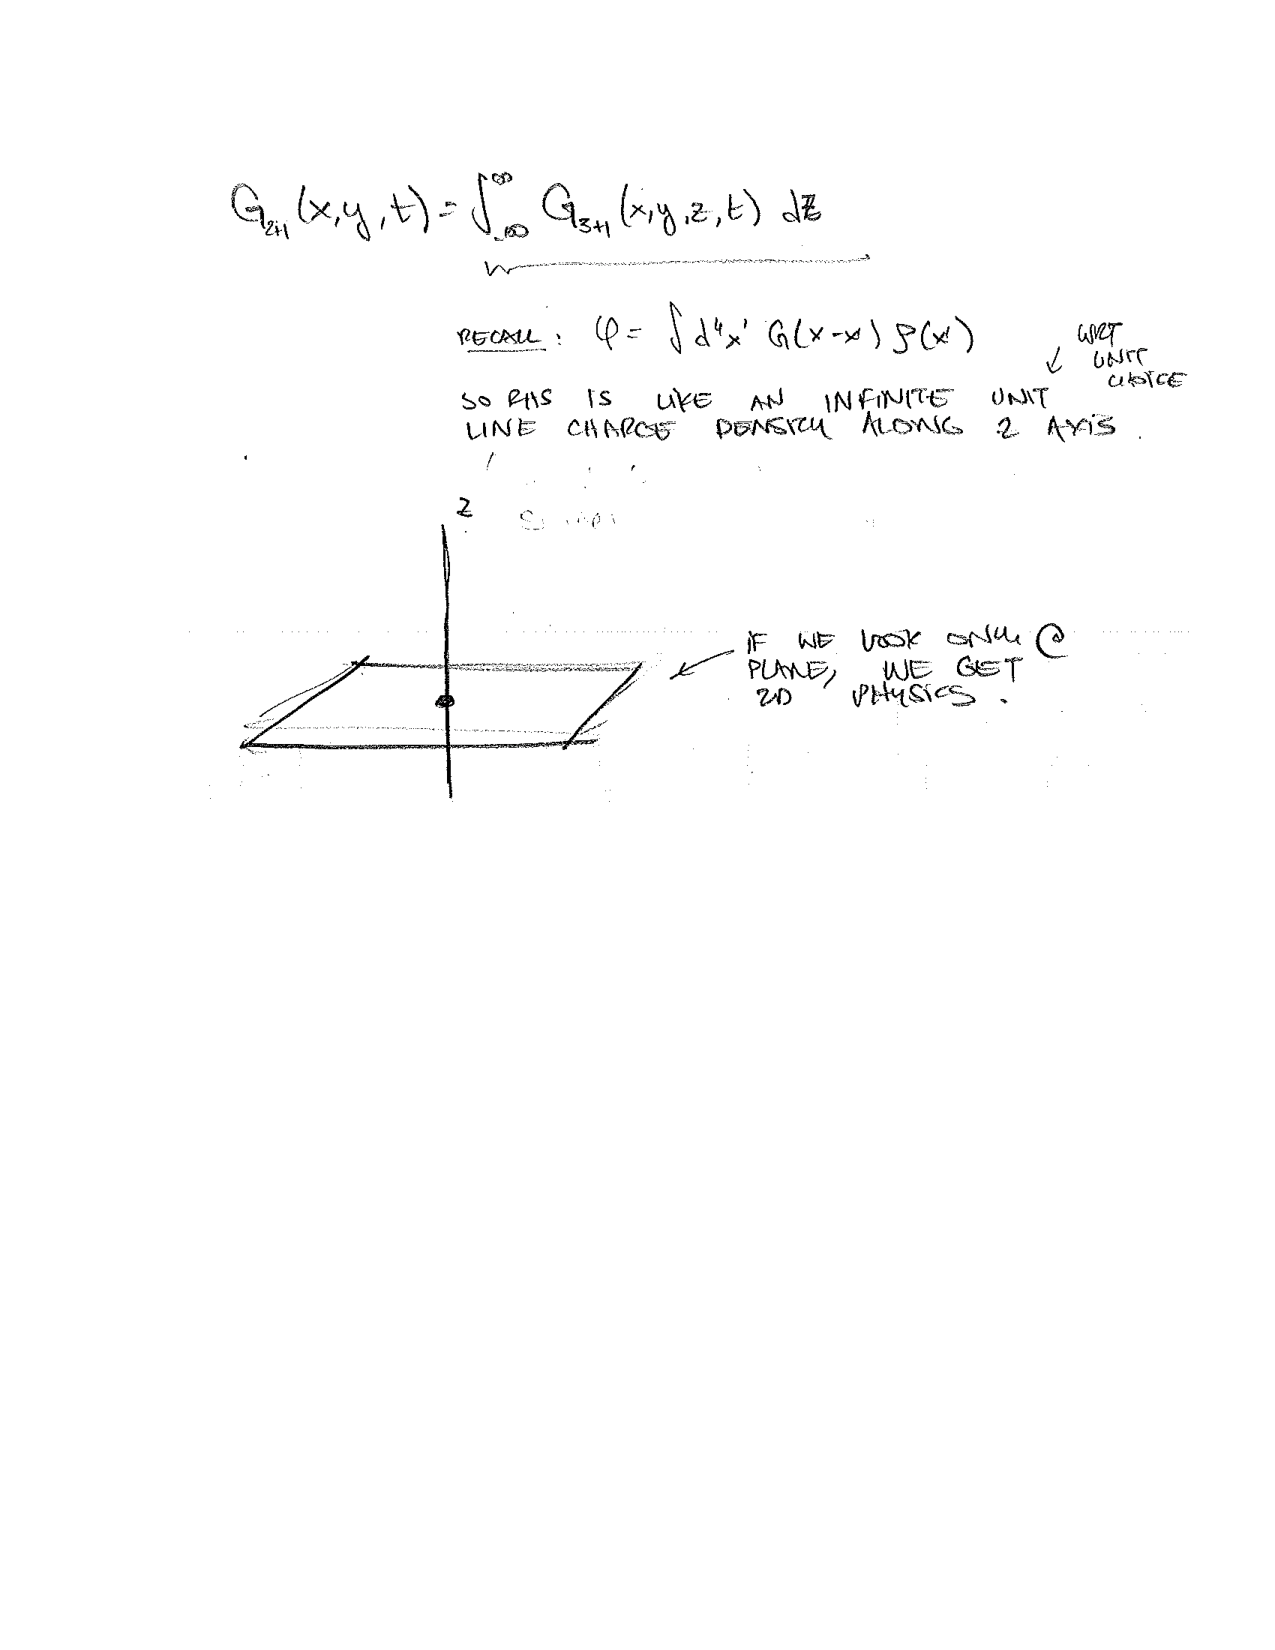
\includegraphics[width=.47\textwidth]{figures/Lec08_XD_2D1}
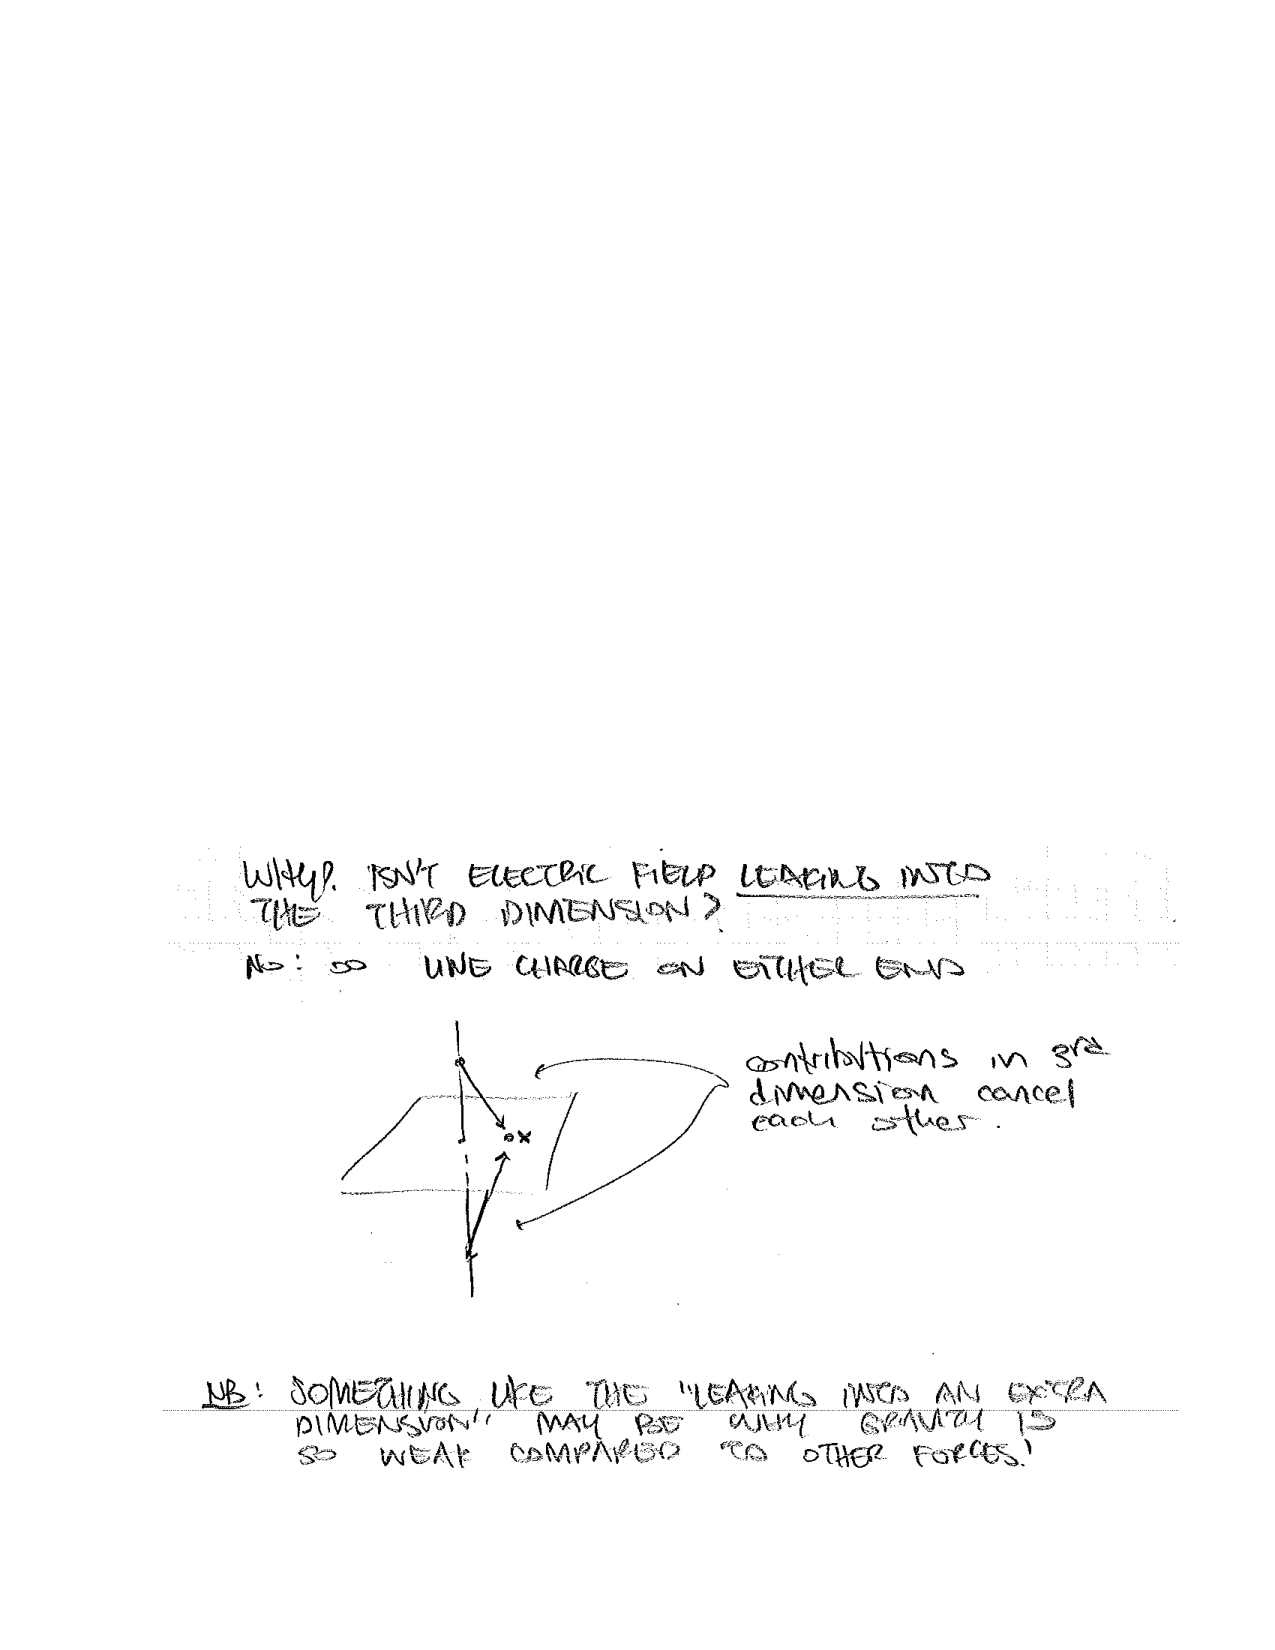
\includegraphics[width=.47\textwidth]{figures/Lec08_XD_2D2}
\end{center}
The key insight is that $\int dz\, G_{(3+1)}$ is precisely the form of the potential coming from an infinite, uniform line charge extending in the $z$-direction from the origin. The electric field would ordinarily `leak' into the extra dimension, but the infinite line charge cancels the potential that leaks off of a given sheet. Note that by symmetry the non-trivial potential profile is restricted to the plane.





%% MOVED TO Lec-09
% \section{A theoretical digression}

% If you'll permit one further digression, let me remind you that the reason why we spend so much time solving for the second derivative is that our models of physics tend to be local. Consider the action, $S = \int dt \, L$. If we have some state $q$ that propagates in spacetime, the natural form of the action is actually an integral with respect to a Lagrangian \emph{density},
% \begin{align}
% 	S = \int d^4x \mathcal L = \int d^4x \left(\text{const.} + q + \partial_\mu q + \cdots\right) \ ,
% \end{align}
% where on the right-hand side we just started writing out all possible polynomials of $q(x,t)$ and the four-derivative $\partial_\mu$. If you have been paying close attention, you'll notice that by writing $q(x,t)$ I have surreptitiously passed from $q$ being a `particle' to being a `field'. We only use $\partial_\mu$ instead of $d/dt$ or $\nabla$ because we expect the theory to be Lorentz invariant\footnote{If your theory is not Lorentz invariant, then replace `Lorentz' with whatever symmetries your system does have. If it has no appreciable symmetries, then may Boltzmann have mercy on your soul.}. In fact, we probably don't want to have any terms that have any free indices like $\partial_\mu q$ because that means it transforms like a Lorentz vector and thus the term is not Lorentz invariant. Furthermore, we can use field redefinitions to remove linear terms\footnote{This is not an obvious statement in the action, but the variation of the action usually comes from a path integral, where on varies over $q(x,t)$. Shifting $q(x,t)$ is like integrating $dx$ versus $d(x+3) = dx$.}. Subject to symmetries, the action looks like:
% \begin{align}
% S = \int d^4x \left[\frac{1}{2}q\left(\partial^2 + \omega_0^2\right)q + cq^3 + dq^4 + e\partial^2 q^2 + \cdots \right]	 \ .
% \end{align}
% You may recognize that the term in parenthesis is simply the `harmonic oscillator' (or wave equation, they're all the same to me) operator, $\mathcal O$. Indeed, when you vary that part of action by itself, you end up with the appropriate differential equation, $\mathcal O q = 0$. 

% What about the other terms? First we should do a bit of dimensional analysis. For my own sanity, let's use natural units where we set $c=\hbar =1$ and all units are measure in mass dimension:
% \begin{align}
% 	[x] = [t] &= -1 \ .
% \end{align}
% This means that $[d^4x] = -4$. Since the action is dimensionless in natural units---after all, it shows up in a $e^{iS}$---then we know the Lagrangian density has dimension $[\mathcal L] = +4$. Since $[\partial]=+1$, we deduce that the variable $q$ has mass dimension $[q]=+1$. Ok, with that in mind, we can look at the `higher order' terms. The coefficients of these terms must have some \emph{negative} mass dimension:
% \begin{align}
% 	c\, , d\, , e \, , \cdots = \left(\frac{1}{M}\right)^n \ ,
% \end{align}
% where $n$ is a positive integer. We've written the mass scale as $M$. Any mass scale in the theory must have physical significance. We could question whether the mass scale $M$ is big or small compared to either $\omega_0$ or the characteristic energies at which we are studying the system. If $M$ is small, then these coefficients are large, and their dynamics are important. However, if we include these terms in our dynamics, then the equations of motion become very nonlinear:
% \begin{align}
% 	\mathcal O q + 3cq^2 + 4d q^3 + \cdots = 0 \ .
% \end{align}
% That would mean that the wave equation approximation is quite bad. By the way, those terms are also clearly non-linear. If we see physics that is approximately described by the wave equation, then these coefficients must be small. We thus expect $M$ to be large---it is an ultraviolet scale. 

% What we intuit is that the scale $M$ is some energy scale where our theory is breaking down. If, for example, we were to \emph{experimentally}\footnote{In the \emph{gedanken} sense.} study this system at energies $E\sim M$, we expect that the effect of these non-linear terms are no longer small and become significant. In other words, the scale $M$ plays the role of a \emph{cutoff} at which our theory described by the linear operator $\mathcal O$ breaks down. For energies well below $M$, we can study the linear system and do \emph{perturbation theory} to study the first few non-linear coefficients that have coefficients that go like $(1/M)$ to a relatively small power. In the regime where our experiment has characteristic energy $E\ll M$, the in-principle infinite number of higher-order coefficients are negligible because we expect those effects to go like $(E/M)^n$; so keeping the first few should be an accurate description of the system.

% This is the notion of an \textbf{effective theory}. All physical models are effective theories. We're simply parameterizing our ignorance about the universe and working in a regime where we are predictive. The effective theory philosophy explains why we are so obsessed with Green's functions of second-derivative operators:
% \begin{itemize}
% 	\item Constant operators are trivial, they're not even differential.
% 	\item Operators with a single derivative are not Lorentz invariant. (The exceptions, like the diffusion operator, are only valid in the non-relativistic regime.)
% 	\item Operators with three, five, or any odd number of derivatives are not Lorentz invariant. They are also suppressed by inverse powers of the cutoff, $M$.
% 	\item Operators that are nonlinear, i.e.~terms in the Lagrangian density that have more than four powers of $q(x,t)$, are also suppressed by inverse powers of the cutoff $M$.
% \end{itemize}
% This tells you that in (3+1)-dimensions, the most interesting non-linear terms are $\mathcal L \supset cq^3+ dq^4$. If you assume that your theory has some $q\to -q$ symmetry, then you can even remove the $c$ term. By the way, this is how you build theories: you start with the most general $\mathcal L$ with an infinite number of terms. Then you argue based on symmetries and the relevance of high-dimensional operators which terms you can throw out. The result is that any reasonable theory in (3+1)-dimensions should be some perturbation of the harmonic oscillator/wave/Poisson system.

% Let me layer onto this a bit more: implicit in writing out $S=\int d^4x\mathcal L$ is the idea that our theory should be manifestly \emph{local}. When we write terms like $q^3$, we really mean $q(x,t)q(x,t)q(x,t)$ at the \emph{same} spacetime point. If this were not true, then the theory would be non-local and the causal structure of the theory would depend on the reference frame. This, in turn would put causality and Lorentz invariance at odds with one another and you'd have to pick one but not both. Some recent alternative formulation of quantum physics based on amplitudes (and not Lagrangians) have proposed that by giving up on \emph{manifest} locality, there may be more elegant descriptions of a theory. Those descriptions are local, they're just not obviously so.

% \begin{exercise}
% If we lived in Flatland, then the action would take the form $S = \int d^3x \mathcal L$. How does the power counting change for a state $q$? How does it change for a general number of spatial dimensions, $D$? Note: quantum effects can change the story quite a bit in $D=1$ and $D>3$. That's different story
% \end{exercise}

% \begin{exercise}
% The Lagrangian density for electrodynamics is
% \begin{align}
% 	\mathcal L = \frac{1}{4}F^{\mu\nu}F_{\mu\nu} \ ,
% \end{align}
% where $F_{\mu\nu}$ is the field strength tensor. Write out the corresponding equations of motion. Notice that you only get half of Maxwell's equations. Where does the other half come from? \textsc{Answer} (partial): the other half of Maxwell's equations come from the geometry of that system. It's most clear in the language of differential forms, but then one has to build up that mathematical machinery.
% \end{exercise}


% % potential future topic: fields from springs












